\section{Experimental Setup}
In this section we describe our experimental setup to evaluate the scalability of distributed training and investigate techniques to accelerate training by leveraging approximations. 
\subsection{TensorFlow}
TensorFlow (~\cite{tensorflow}) is a machine learning system that is designed to operate at large scale across numerous heterogeneous distributed systems. TensorFlow using dataflow graphs to represent the desired computation for a machine learning algorithm. TensorFlow allows distributing the computation between different nodes in a distributed system by replicating the dataflow graph across different nodes or partitioning subgraphs of the computation across them. As a result, the computation can be partitioned between different \emph{workers} which may be executed on different nodes. 

The ability of TensorFlow to flexibly distribute computation across numerous nodes, as well as flexibly describe typically used neural networks, makes it a good choice to test the efficiency and challenges of large-scale distributed training. Training neural networks essentially involves processing large amounts of data and \emph{training} models to generate desired labels for each input. This requires computing a \emph{forward pass} operation on each batch of input data and a \emph{backward pass} to compute the gradients and update the parameters of the neural network. To parallelize computation across different \emph{workers}, we partition the training data across multiple nodes, and propogate the gradients computed by each each worker to the network models seen by the other workers (this form of data parallelism is referred to as \emph{data parallelism}). Distributed training requires that multiple workers share the data that form the parameters of the neural network. In order to converge, the updates computed by each worker needs to be propagated to the other workers. The sharing of parameter updates between workers can be done synchronously or asynchronously. TensorFlow allows sharing parameter data between different workers and exchange of updates by using a \emph{parameter server}\cite{parameter_server}. A parameter server runs independently of the workers and serves to synchronize updates from different workers. At the end of each \emph{step}, i.e., when a worker completes a batch of images, the computed gradients are sent to the parameter server to update the parameters of the neural network. The 
updated parameter values which includes updates from different workers is sent back to each worker to use for the next step of training.
TensorFlow provides abstractions to employ parameter servers for distributed training. 

\subsection{Cifar-10}
To perform and evaluate our experiments in distributed training in TensorFlow, we evaluate the image classification task using the CIFAR-10~\cite{cifar10} dataset. Image classification involves classifying each image into a predecided set of classes of objects. The CIFAR-10 dataset consists of 60000 32x32 colour images in 10 classes, with 6000 images per class. There are 50000 training images and 10000 test images. The dataset is divided into five training batches and one test batch, each with 10000 images. The test batch contains exactly 1000 randomly-selected images from each class. The training batches contain the remaining images in random order, but some training batches may contain more images from one class than another. Between them, the training batches contain exactly 5000 images from each class. 

The neural network comprises of nine layers with five of them being trainable (the convolutional, softmax and fully connected layers). The layer architecture for CIFAR-10 is depicted in Figure \ref{fig:cifar10}

\begin{figure}[h]
\centering
  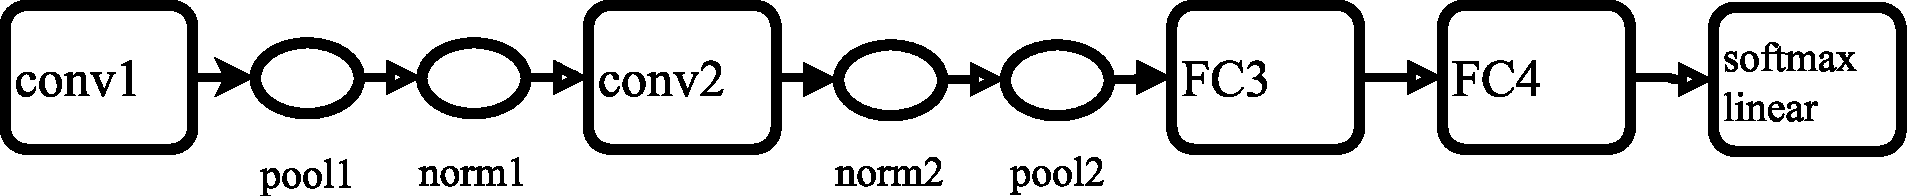
\includegraphics[keepaspectratio,width=\columnwidth]{figures/Cifar10_tensorflow.pdf}
  \caption{\textbf{Layers in the CIFAR-10 network}}
  \label{fig:cifar10}
\end{figure}

\subsection{Distributed System Infrastructure}

For running distributed training we used the cluster
at Intel Research Pittsburgh. The cluster consists 
of 150 servers nodes with the number of computing
cores claimed to be more than 1000 \cite{tashi}.
Figure \ref{fig:bigdata} provides details about the
different compute platforms and the network
bandwidth available. The cluster uses a virtual machine
managment system \cite{tashi} that allows creation of different Virtual
Machines on different racks.

\begin{figure}[h]
\centering
  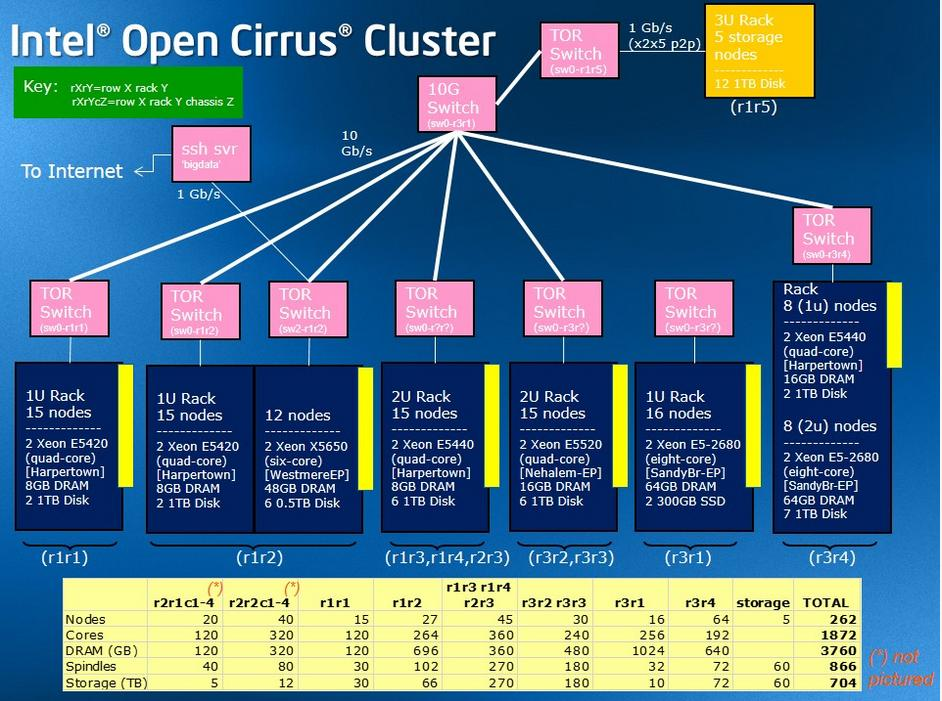
\includegraphics[keepaspectratio,width=\columnwidth]{figures/bigdata.jpg}
  \caption{\textbf{Cluster at Intel Research Pittsburgh\cite{bigdatafig}}}
  \label{fig:bigdata}
\end{figure}



